\documentclass[border=10pt]{standalone}
\usepackage{amsmath}
\usepackage{pgfplots}
\pgfplotsset{compat=1.17}
\begin{document}
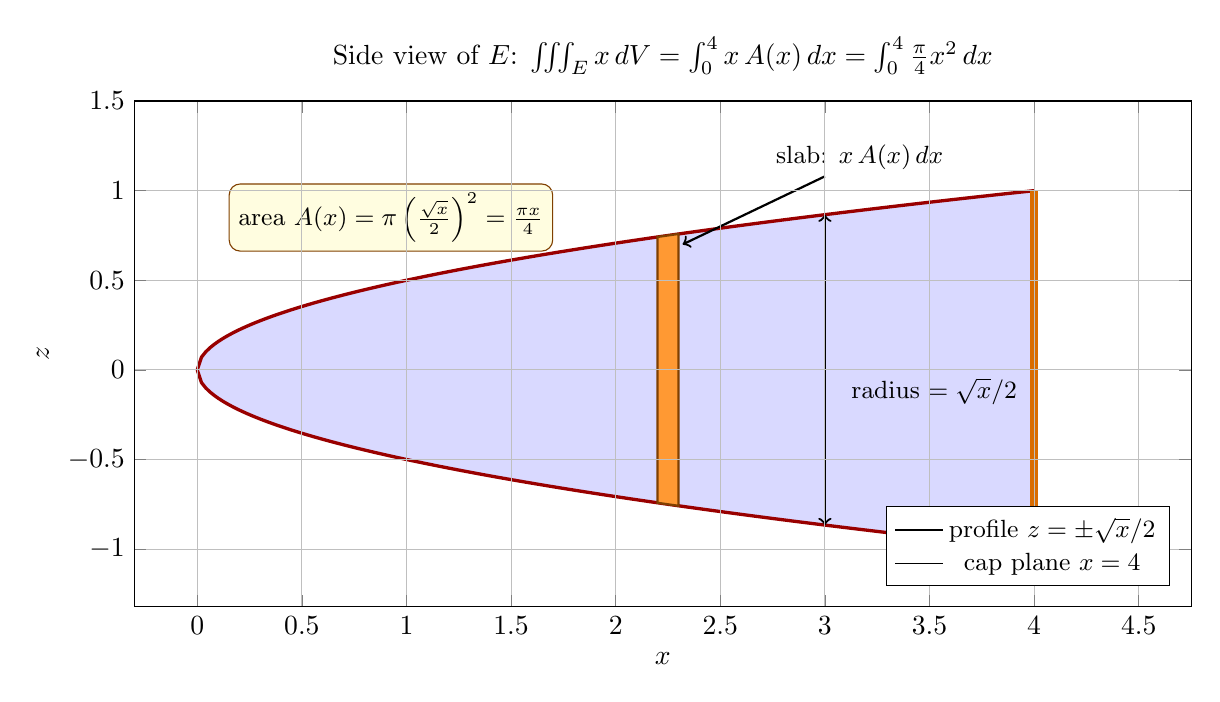
\begin{tikzpicture}
\begin{axis}[
    width=15cm, height=8cm,
    xlabel={$x$}, ylabel={$z$},
    xmin=-0.3, xmax=4.75, ymin=-1.32, ymax=1.5,
    grid=major, axis on top,
    title={Side view of $E$:  $\iiint_E x\,dV=\int_0^4 x\,A(x)\,dx=\int_0^4 \frac{\pi}{4}x^2\,dx$},
    legend style={at={(0.98,0.04)}, anchor=south east, font=\small},
]
% fills (no stroke) above and below the x-axis
\addplot[domain=0:4, samples=200, draw=none, fill=blue!15] {sqrt(x)/2} \closedcycle;
\addplot[domain=0:4, samples=200, draw=none, fill=blue!15] {-sqrt(x)/2} \closedcycle;
% profile curves (stroke only)
\addplot[red!60!black, very thick, domain=0:4, samples=200] {sqrt(x)/2};
\addplot[red!60!black, very thick, domain=0:4, samples=200] {-sqrt(x)/2};
% cap plane x = 4
\addplot[orange!85!black, line width=3pt] coordinates {(4,-1) (4,1)};
% slab of thickness dx at x = 2.25
\filldraw[fill=orange!80, draw=orange!50!black, thick]
    (axis cs:2.2,-0.7416) -- (axis cs:2.2,0.7416) -- (axis cs:2.3,0.7583) -- (axis cs:2.3,-0.7583) -- cycle;
% radius arrow at x = 3
\draw[<->, thick] (axis cs:3,-0.866) -- (axis cs:3,0.866);
\node[anchor=west, font=\small] at (axis cs:3.08,-0.12) {radius $=\sqrt{x}/2$};
% annotations
\node[draw=orange!50!black, fill=yellow!12, rounded corners, font=\small, anchor=west]
    at (axis cs:0.15,0.85) {area $A(x)=\pi\left(\frac{\sqrt{x}}{2}\right)^{2}=\frac{\pi x}{4}$};
\draw[->, thick] (axis cs:3.0,1.08) -- (axis cs:2.32,0.7);
\node[anchor=south west, font=\small] at (axis cs:2.72,1.06) {slab: $x\,A(x)\,dx$};
% axes through origin
\addplot[black, thin] coordinates {(-0.3,0) (4.75,0)};
\addplot[black, thin] coordinates {(0,-1.32) (0,1.5)};
\legend{profile $z=\pm\sqrt{x}/2$, cap plane $x=4$}
\end{axis}
\end{tikzpicture}
\end{document}